%**************************************************************************************
% License:
% CC BY-NC-SA 4.0 (http://creativecommons.org/licenses/by-nc-sa/4.0/)
%**************************************************************************************

\documentclass[notes]{beamer}

\mode<presentation> {

\usetheme{Madrid}

% Burnt orange
\definecolor{burntorange}{rgb}{0.8, 0.33, 0.0}
\colorlet{beamer@blendedblue}{burntorange}
% Pale yellow
\definecolor{paleyellow}{rgb}{1.0, 1.0, 0.953}
\setbeamercolor{background canvas}{bg=paleyellow}
% Secondary and tertiary palett
\setbeamercolor*{palette secondary}{use=structure,fg=white,bg=burntorange!80!black}
\setbeamercolor*{palette tertiary}{use=structure,fg=white,bg=burntorange!60!black}

% To remove the footer line in all slides uncomment this line
%\setbeamertemplate{footline}
% To replace the footer line in all slides with a simple slide count uncomment this line
%\setbeamertemplate{footline}[page number]

% To remove the navigation symbols from the bottom of all slides uncomment this line
%\setbeamertemplate{navigation symbols}{}
}

\usepackage{amsmath}
\usepackage{bm}
\usepackage{breqn}
\usepackage{cancel}
\usepackage{graphicx} % for figures
\usepackage{subcaption} % for subplots 
\usepackage[labelsep=space,tableposition=top]{caption}
\renewcommand{\figurename}{Fig.} 
\usepackage{cleveref}
\usepackage{caption,subcaption}% http://ctan.org/pkg/{caption,subcaption}
\usepackage{booktabs} % Allows the use of \toprule, \midrule and \bottomrule in tables
\usepackage{multirow}

% To print 2 slides on a page
%\usepackage{handoutWithNotes}
%\pgfpagesuselayout{2 on 1}[border shrink=2mm]
%----------------------------------------------------------------------------------------
%	TITLE PAGE
%----------------------------------------------------------------------------------------
% The short title appears at the bottom of every slide, the full title is only on the title page
\title[CE394M: Linear Elasticity]{CE394M: Linear Elasticity} 
\author{Krishna Kumar} % name
\institute[UT Austin] % institution 
{
University of Texas at Austin \\
\medskip
\textit{
  \url{krishnak@utexas.edu}} % Your email address
}
\date{\today} % Date, can be changed to a custom date

\begin{document}

\begin{frame}
\titlepage % title page as the first slide
\end{frame}

\begin{frame}
 % Table of contents slide, comment this block out to remove it
 \frametitle{Overview}
  %Throughout your presentation, if you choose to use \section{} and \subsection{} 
  %commands, these %will automatically be printed on this slide as an overview 
 \tableofcontents
\end{frame}

%----------------------------------------------------------------------------------------
% slides
%----------------------------------------------------------------------------------------
\section{Linear Elasticity}
%----------------------------------------------------------------------------------------
\begin{frame}
\frametitle{Isotropic linear elastic stress-strain relations}
The linear relationship between the stress and strain tensor is a linear one. The stress component
is a linear combination of the strain tensor:
\begin{equation*}
	\begin{split}
		\sigma_{ij} = C_{ij11}\varepsilon_{11} + C_{ij12}\varepsilon_{12} + C_{ij13}\varepsilon_{13} + \\
			C_{ij21}\varepsilon_{21} + C_{ij22}\varepsilon_{22} + C_{ij23}\varepsilon_{23} + \\ C_{ij31}\varepsilon_{31} + C_{ij32}\varepsilon_{32} + C_{ij33}\varepsilon_{33}
	\end{split}
\end{equation*} 
The most general form for \textit{linear} stress-strain relations for a \textit{Cauchy elastic}
material is given by:
\mode<beamer>{
	\begin{equation*}
		\sigma_{ij} = B_{ij} + C_{ijkl} \varepsilon_{kl}
	\end{equation*}
}
\mode<handout>{
	\vspace{1cm}
} 
	Where $B_{ij}$ is the components of initial stress tensor corresponding to the initial strain free (when all strain components $\varepsilon_{kl} = 0$). $C_{ijkl}$ is the tensor of material \textit{elastic constants}.
	
	If it is assumed that the initial strain free state corresponds to an \textit{initial stress free state}, that is $B_{ij} = 0$, the equations reduces to:
\mode<beamer>{	
	\begin{equation*}
		\sigma_{ij} = C_{ijkl} \varepsilon_{kl}
	\end{equation*}
}  
\mode<handout>{
	\vspace{1.5cm}
} 
\end{frame}

%----------------------------------------------------------------------------------------
\begin{frame}
\frametitle{Observation on linear elasticity}
\mode<beamer>{
	\begin{enumerate}
		\item $\sigma_{ij} = C_{ijkl} \varepsilon_{kl}$ is a general expression relating stress to strains for a linear solid.
		\item $C_{ijkl}$ is a 4th order tensor containing 81 terms (we trick using symmetry and reduce order).
		\item $C_{ijkl}$ material response functions having dimensions $F/L^2$.
		\item Homogeneous: $C_{ijkl}$ independent of position
		\item Isotropic: $C_{ijkl}$ independent of frame of reference.
		\item Because the stress is symmetric: $\sigma_{ij} = \sigma_{ji}$, $C_{ijkl} = C_{jikl}$. Strain is symmetric $\varepsilon_{kl} = \varepsilon_{lk}$ and $C_{ijkl} = C_{ijlk}$. Hence the number of independent variables drop from 81 to 36. 
		\item Both the stress and the strain tensor have only 6 independent values, therefor write them as vecotrs, then the stiffness tensor can be written as a matrix (compromise I can not rotate tensor).
	\end{enumerate}
}
\mode<handout>{
	\vspace{1cm}
}
\end{frame}

%----------------------------------------------------------------------------------------
\begin{frame}
\frametitle{Stress-strain relationship}
\begin{equation*}
\begin{bmatrix}
	\sigma_{11} \\
	\sigma_{22} \\
	\sigma_{33} \\
	\sigma_{12} \\
	\sigma_{23} \\
	\sigma_{31} \\
\end{bmatrix} %
= %
\begin{bmatrix}
	C_{11} & C_{12} & C_{13} & C_{14} &   C_{15} & C_{16}\\
	C_{21} & C_{22} & C_{23} & C_{24} &   C_{25} & C_{26}\\
	C_{31} & C_{32} & C_{33} & C_{34} &   C_{35} & C_{36}\\
	C_{41} & C_{42} & C_{43} & C_{44} &   C_{45} & C_{46}\\
	C_{51} & C_{52} & C_{53} & C_{54} &   C_{55} & C_{56}\\
	C_{61} & C_{62} & C_{63} & C_{64} &   C_{65} & C_{66}\\
\end{bmatrix} %
\begin{bmatrix}
\varepsilon_{11} \\
\varepsilon_{22} \\
\varepsilon_{33} \\
\varepsilon_{12} \\
\varepsilon_{23} \\
\varepsilon_{31} \\
\end{bmatrix}
\end{equation*}
$C_{ijkl}$ is a tensor of material \textit{elastic constants}. However, the above $[\mathbf{C}]$ is not a tensor anymore. So we can not rotate the matrix to another frame of reference. This relationship is useful for isotropic materials, where $\mathbf{C}$ is independent of the frame of reference. 
\mode<beamer>{
	\begin{equation*}
		\left\{\sigma\right\} = \left[\mathbf{C}\right]\left\{\varepsilon\right\}
	\end{equation*}
}
\mode<handout>{
	\vspace{1cm}
}
The inverse of the relationship (Compliance matrix): 
\mode<beamer>{
	\begin{equation*}
	\left\{\varepsilon\right\} = \left[\mathbf{D}\right]\left\{\sigma\right\}
	%
	\qquad 
	%
	 \left[\mathbf{D}\right] = \left[\mathbf{C}\right]^{-1}
	\end{equation*}
}
\mode<handout>{
	\vspace{1cm}
}
\end{frame}

%----------------------------------------------------------------------------------------
\begin{frame}
\frametitle{Isotropic Linear Elastic Stress-strain relationship}
The \textit{isotropic tensor} $C_{ijkl}$:
\begin{equation*}
C_{ijkl} = \lambda \delta_{ij}\delta_{kl} + \mu (\delta_{ik}\delta_{jl} + \delta_{il}\delta_{jk}) + \alpha (\delta_{ik}\delta_{jl} - \delta_{il}\delta_{jk})
\end{equation*}
Where $\lambda, \mu, \text{ and }, \alpha$ are scalar constants. Since $C_{ijkl}$ must satisfy symmetry, $\alpha = 0$.
\mode<beamer>{
	\begin{equation*}
	C_{ijkl} = \lambda \delta_{ij}\delta_{kl} + \mu (\delta_{ik}\delta_{jl} + \delta_{il}\delta_{jk})
	\end{equation*}
}
\mode<handout>{
	\vspace{1cm}
}
So the stress:
\mode<beamer>{
	\begin{align*}
	\sigma_{ij} & = \lambda \delta_{ij}\delta_{kl}\varepsilon_{kl} + \mu (\delta_{ik}\delta_{jl} + \delta_{il}\delta_{jk})\varepsilon_{kl}\\
	\sigma_{ij} & = \lambda \varepsilon_{kk} \delta_{ij} + 2\mu \varepsilon_{ij}
	\end{align*}
}
\mode<handout>{
	\vspace{2.5cm}
}
Hence for an isotropic linear elastic material, there are only two independent material constants, $\lambda$ and $\mu$, which are called \textit{Lame's constants}.
\end{frame}

%----------------------------------------------------------------------------------------
\begin{frame}
\frametitle{Hooke's law}
\noindent
\fboxsep=0pt
\noindent
\begin{minipage}[t]{0.89\linewidth}
	Empirical observation:
	\mode<beamer>{
		\begin{equation*}
			\Delta \varepsilon_a = \Delta \sigma_{axial} \cdot \frac{1}{E} \rightarrow \Delta \varepsilon_{11} = \frac{\Delta \sigma_{11}}{E}
		\end{equation*}
	}
	\mode<handout>{
		\vspace{1.5cm}
	}
	Where $E$ is defined as the \textit{Young's modulus}.

	The lateral strains are defined as:
	\mode<beamer>{
		\begin{align*}
			\Delta \varepsilon_{22} & = - \nu \Delta \varepsilon_{11} \\
			\Delta \varepsilon_{33} & = - \nu \Delta \varepsilon_{11}
		\end{align*}
	}
	\mode<handout>{
		\vspace{2cm}
	}

	Using superposition for principal stresses:
		\begin{align*}
			\varepsilon_{11} & = (1/E)\left[\sigma_{11} - \nu \sigma_{22} -\nu \sigma_{33}\right] \\
			%
			\varepsilon_{22} & = (1/E)\left[-\nu \sigma_{11} + \sigma_{22} -\nu \sigma_{33}\right] \\
			%
			\varepsilon_{33} & = (1/E)\left[-\nu \sigma_{11} - \nu \sigma_{22} + \sigma_{33}\right]
		\end{align*}
\end{minipage}%
\hfill%
\begin{minipage}[t]{0.1\linewidth}
	\begin{figure}
		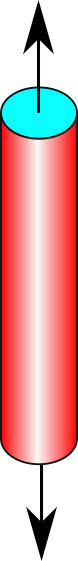
\includegraphics[width=\textwidth]{figs/hookes-law.png}
	\end{figure}
\end{minipage}	
\end{frame}

%----------------------------------------------------------------------------------------
\begin{frame}
\frametitle{Hooke's law}

\begin{equation*}
	\begin{Bmatrix}
		\varepsilon_{11}\\
		\varepsilon_{22}\\
		\varepsilon_{33}\\
	\end{Bmatrix} = \frac{1}{E}
	\begin{bmatrix}
		1 & -\nu & -\nu \\
		-\nu & 1 & -\nu \\
		-\nu & -\nu & 1 \\
	\end{bmatrix}
	\begin{Bmatrix}
		\sigma_{11}\\
		\sigma_{22}\\
		\sigma_{33}\\
	\end{Bmatrix}
\end{equation*}

It is possible to invert the matrix to obtain the generalized Hooke's law: \mode<beamer>{$[\sigma] = [\mathbf{C}][\varepsilon]$.}

\begin{equation*}
	\begin{Bmatrix}
		\sigma_{11}\\
		\sigma_{11}\\
		\sigma_{11}\\
		\sigma_{11}\\
		\sigma_{11}\\
		\sigma_{11}\\
	\end{Bmatrix} = \alpha
	\begin{bmatrix}
		(1-\mu) & \nu & \nu & 0 & 0 & 0 \\
	   			& (1-\nu) & \nu & 0 & 0 & 0 \\
	   			&  & (1-\nu) & 0 & 0 & 0 \\
	   			&  & & \frac{(1-2\nu)}{2} & 0 & 0 \\
	   			&  & & & \frac{(1-2\nu)}{2}  & 0 \\
	   			&  & & & & \frac{(1-2\nu)}{2} \\
	\end{bmatrix}
	\begin{Bmatrix}
		\varepsilon_{11}\\
		\varepsilon_{22}\\
		\varepsilon_{33}\\
		2\varepsilon_{12}\\
		2\varepsilon_{13}\\
		2\varepsilon_{23}\\
	\end{Bmatrix}
\end{equation*}
Where $\alpha = E / ((1+\mu)(1-2\mu))$.
Similarly, we can obtain the inverse matrix.
\end{frame}


%----------------------------------------------------------------------------------------
\begin{frame}
\frametitle{Hooke's law}
The matrices $[\mathbf{C}]$ and $[\mathbf{D}]$ contains two indepdent variables $E$ and $\mu$, where $E > 0$ and $-1 \le \mu \le 0.5$. 
The matrix can also be defined in terms of Lame's constants.
\begin{equation*}
	\begin{cases}
		\lambda = \frac{E \nu}{(1+\nu)(1-2\nu)} \quad \text{Lame's modulus (wave propagation)}\\
		\mu = G = \frac{E}{2(1+\nu)}
		\quad \text{Shear modulus (shear behavior)}\\
		K = \frac{E}{3(1-2\nu)}
		\quad \text{Bulk modulus (volumetric behavior)}\\
	\end{cases}
\end{equation*}
\end{frame}

%----------------------------------------------------------------------------------------
\begin{frame}
\frametitle{Isotropic linear elastic}
	\begin{figure}
		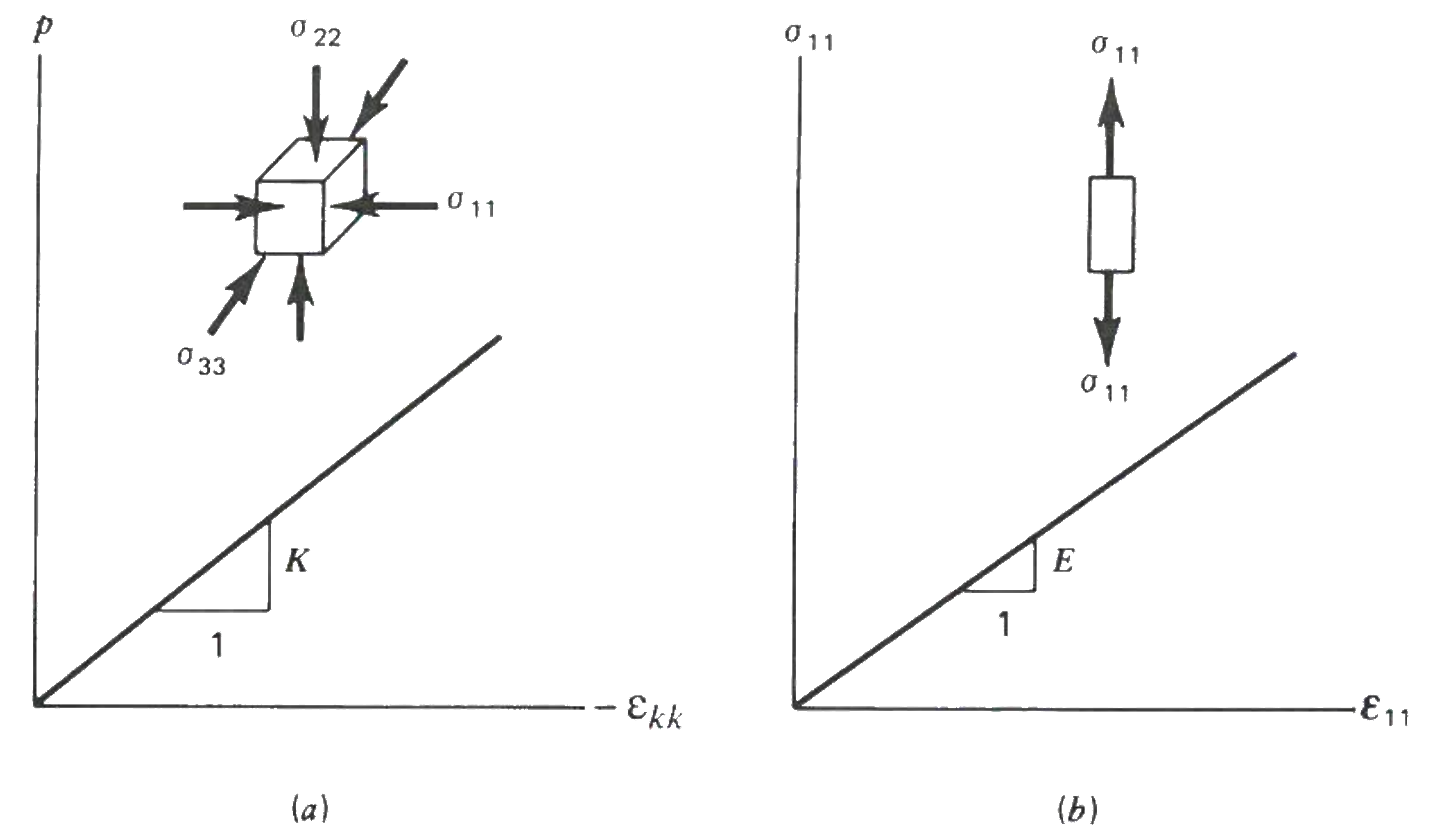
\includegraphics[width=0.95\textwidth]{figs/isotropic-linear-elastic.png}
		\caption*{Behavior of isotropic linear elastic material in simple tests: (a) hydrostatic compression test ($\sigma_{11} = \sigma_{22} = \sigma_{33} = p$) and (b) simple tension test (Chen 1994)}
	\end{figure}
\end{frame}

%----------------------------------------------------------------------------------------
\begin{frame}
\frametitle{Isotropic linear elastic}
\textbf{Hydrostatic compression test}
The non-zero components of stress: \mode<beamer>{$\sigma_{11} = \sigma_{22} = \sigma_{33} = -p = \sigma_{kk}/3$.}

The \textit{Bulk modulus, K,}  is defined as the ratio between the \textit{hydrostatic pressure p} nd the corresponding volume change $\delta \varepsilon_v = \varepsilon_{kk}$. 
\mode<beamer>{	
	\begin{equation*}
		K = - \frac{p}{\varepsilon_{kk}} = \lambda + \frac{2}{3}\mu
	\end{equation*}
}  
\mode<handout>{
	\vspace{1.5cm}
} 
\textbf{Simple tension test}
The only non-zero components of stress: \mode<beamer>{$\sigma_{11} = \sigma$}

The \textit{Young's modulus, K,}  is defined as the ratio between the \textit{hydrostatic pressure p} nd the corresponding volume change $\Delta \varepsilon_v = \varepsilon_{kk}$. 
\mode<beamer>{	
	\begin{equation*}
	K = - \frac{p}{\varepsilon_{kk}} = \lambda + \frac{2}{3}\mu
	\end{equation*}
}  
\mode<handout>{
	\vspace{1.5cm}
}
\end{frame}

%----------------------------------------------------------------------------------------
\begin{frame}
\frametitle{Isotropic linear elastic}
\begin{figure}
	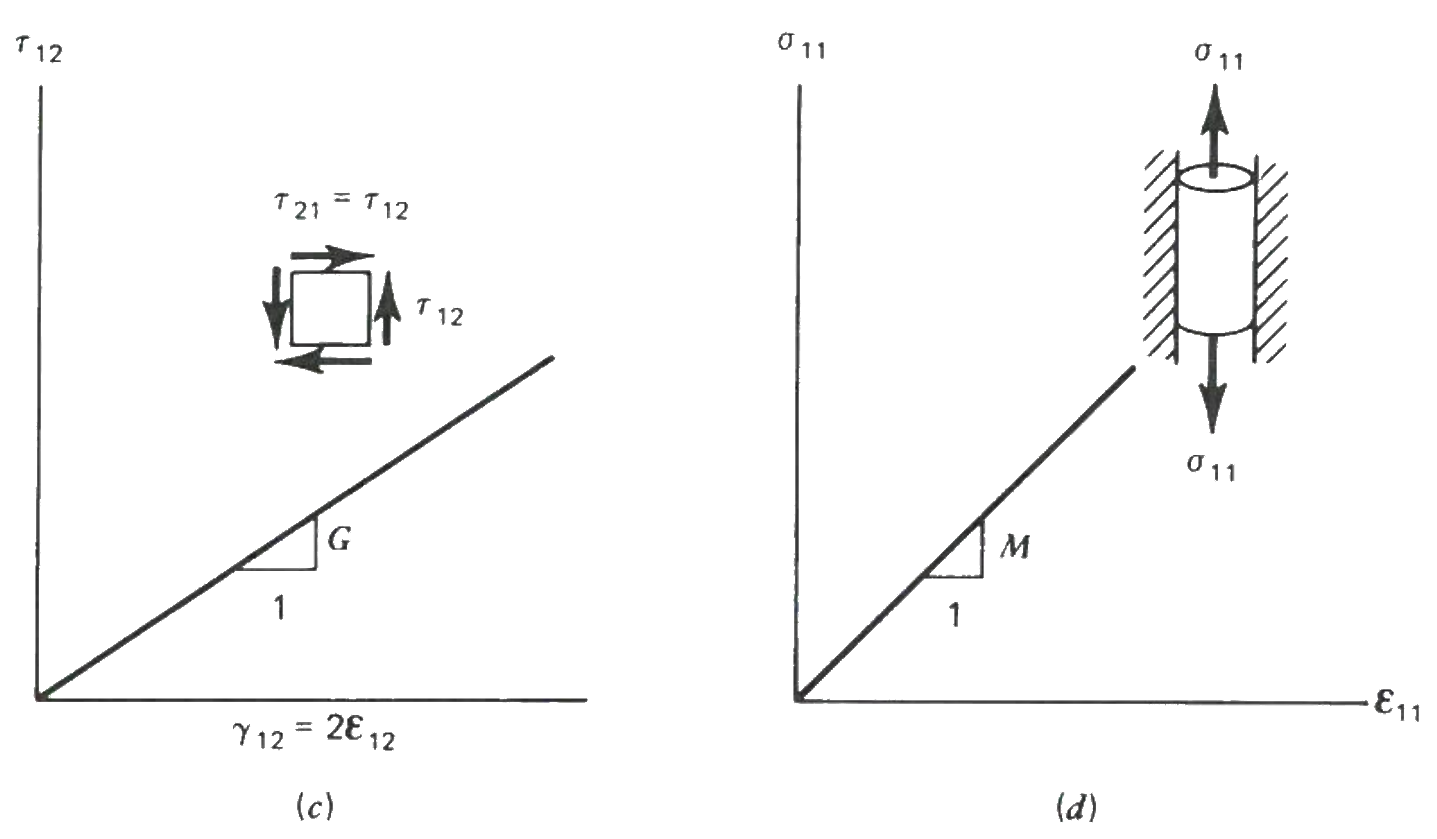
\includegraphics[width=0.95\textwidth]{figs/isotropic-linear-elastic-1.png}
	\caption*{Behavior of isotropic linear elastic material in simple tests: (c) pure shear test, and (d) uniaxial strain test (Chen 1994)}
\end{figure}
\end{frame}

%----------------------------------------------------------------------------------------
\begin{frame}
\frametitle{Isotropic linear elastic}
\textbf{Simple shear test}

The non-zero components of stress: \mode<beamer>{$\sigma_{12} = \sigma_{21} = \tau_{12} = \tau_{21} = \tau$.}

The \textit{Shear modulus, $G$ or $\mu$,}  is defined as: 
\mode<beamer>{	
	\begin{equation*}
	G = \mu = \frac{\sigma_{12}}{\gamma_{12}} = \frac{\tau}{2\varepsilon_{12}}
	\end{equation*}
}  
\mode<handout>{
	\vspace{1.5cm}
}

\textbf{Uniaxial strain test}
The test is carried out by applying a uniaxial stress component $\sigma_{11}$ in the axial direction of a cylindrical sample, whose lateral surface is \textit{restrained} against lateral movement (Oedometer test). Axial strain $\varepsilon_11$ is the only nonvanishing component. The \textit{constrained modulus M} or as PLAXIS calls it $E_{oed}$ is defined as the ratio between $\sigma_{11}$ and $\varepsilon_11$.
\mode<beamer>{	
	\begin{align*}
		\sigma_{11} & = \frac{E}{(1+\nu)(1-2\nu)}\left[(1-\nu)\varepsilon_{11} + \nu\cancelto{0}{\varepsilon_{22}} + \nu\cancelto{0}{\varepsilon_{33}}\right] = \frac{E(1-\nu)\varepsilon_{11}}{(1+\nu)(1-2\nu)} \\
		M & = E_{oed} = \frac{\sigma_{11}}{\varepsilon_{11}} = \frac{(1 - \nu)E}{(1+\nu)(1-2\nu)} = (\lambda + 2\mu)
	\end{align*}
}  
\mode<handout>{
	\vspace{1.5cm}
}

\end{frame}


%----------------------------------------------------------------------------------------
\begin{frame}
\frametitle{Plane stress v Plane strain}
For a frame with an axis perpendicular to the plane of interest, $x_3$ or $z$:

\textbf{Plane stress}
\mode<beamer>{$\sigma_{33} = \sigma_{zz} = \tau_{xz} = \tau_{yz} = 0$.}\mode<handout>{\vspace{1cm}.}

The strain in $z$ is written as:
\mode<beamer>{	
	\begin{equation*}
	\varepsilon_{zz} = \frac{-\nu}{E}(\sigma_{xx} + \sigma_{yy}) = \frac{-\nu}{1-\nu}(\varepsilon_{xx} + \varepsilon_{yy}) 
	\end{equation*}
The plane stress are commonly used for thin flat plates loaded in the plane of the plate.
}  
\mode<handout>{
	\vspace{2.5cm}
}


\textbf{Plane strain}
\mode<beamer>{$\varepsilon_{33} = \varepsilon_{zz} = \gamma_{xz} = \gamma_{yz} = 0$.}\mode<handout>{\vspace{1cm}.}

The stress in $z$ is written as:
\mode<beamer>{	
	\begin{equation*}
	\sigma_{zz} = \nu(\sigma_{xx} + \sigma_{yy})
	\end{equation*}
	The plane strains are commonly used for elongated bodies of uniform cross sections subjected to uniform loading along the longitudinal axis (tunnels, dams, retaining walls, soil slopes, etc.).
}  
\mode<handout>{
	\vspace{2.5cm}
}
\end{frame}
\end{document}